\section{TextCaps:Origin}
本文主要的点在于胶囊网络字符识别架构和基于实例化参数扰动的图像数据生成技术,下面将分别进行介绍。

\subsection{ 胶囊网络字符识别架构}
胶囊网络结构:

卷积1 :64个3*3核,stride= 2;

卷积2 :128个3*3核,stride= 1;

卷积3 :256个3*3核,stride= 2;

主要胶囊层 :32通道,8维胶囊,每个胶囊包含8个卷积单元,9*9的核并且stride=2;

特征胶囊层:全连接层,每一类是16维胶囊,有多少类别就对应多少个胶囊。

在主胶囊层和特征胶囊层用动态路由算法,采用三次路由迭代。参考自\cite{sabour2017dynamic}

输入胶囊是数据集$J$,28×28的图像。

输出是一个$J\times M \times28$的张量$C$,包含相关的实例化参数。

每一个$C_j,j\in[J]$是第$j^th$的训练样本的实例化参数矩阵
采用独热编码的形式,在将$C$输入到解码网络之前,只有是这个类的才不为零,其他为零。经过这个操作后,记为$\hat{C}$

特征胶囊层是一个全连接层后面跟着五个反卷积层,该层的输入是$\hat{C}$输出为28×28的图像。在特征胶囊层中除了最后一层是采用sigmoid激活函数,其他层用RELU激活函数。

作者在这种情况下做实验发现,采用大量样本才能获得好的结果。这显然是不行的,同时主胶囊层已经很完美了。问题出在特征胶囊层无法很好的重建。其原因还是在于样本数量不够。因此提出了一种新的训练样本生成方法,它利用胶囊网络中实例化参数的概念来增强原始训练样本

\subsection{基于实例化参数扰动的图像数据生成技术}

因为已经可以提取到足够多的特征,所以可以通过这些特征向量来描述任意字符。通过训练好的模型已经可以通过实例化参数来进行很好的重建了。因此,想在实例化参数中加入一些噪声,以此来产生新的样本。

首先采用原始的包含2000个样本的数据集。为了保证一致性,取每一个类别中的前200个。采用这么多的样本训练胶囊网络。训练结果称为$M_{1,caps},M_{1,dec}$,前面表示主胶囊层,后面表示特征胶囊层。再通过这个网络生成一部分样本,生成样本的过程中保留输入到特征胶囊层的实例化参数。


生成的样本不太清晰,为了解决这个问题,对生成样本进行了锐化。将锐化后的生成样本加上前面的原始样本作为新的数据集再去训练,得到$\widetilde{M_{1,dec}}$。训练这个网络的目的在于为了消除模糊。结束后对这次生成的结果进行挑选。因为会产生一些不符合实际的样本。

最后将这个新的网络$\widetilde{M_{1,dec}}$和之前保留的实例化参数结合,通过对实例化参数中的各个参数进行扰动来生成新的样本。

在对实例化参数进行扰动的时候,作者通过分析选择了对结果影响较大的前两个参数进行扰动。为了使得结果可控,每次只扰动一个参数。每扰动一次,对于每一类生成50个新的随机的样本。对于扰动的幅度作者进行了限制以避免出现无效的图像。


通过这样的方法增加样本量之后,重新训练识别网络,并获得很好的效果。









\subsection{不同的重建损失函数}
作者在此节提出了4种损失函数,分别是MSE,L1 Norm, SSIM,Binary Cross-Entropy (BCE)。并且采用了两两结合的方法。具体来说就是每次生成图像的时候采用两个损失函数生成两张图片,对每张图片的各个像素点与原图进行对比,选择靠近真实点的像素点作为真正的输出。
\subsection{实验结果}
实验结果具体看Table2截图
\begin{figure}[!htbp]
	\centering
	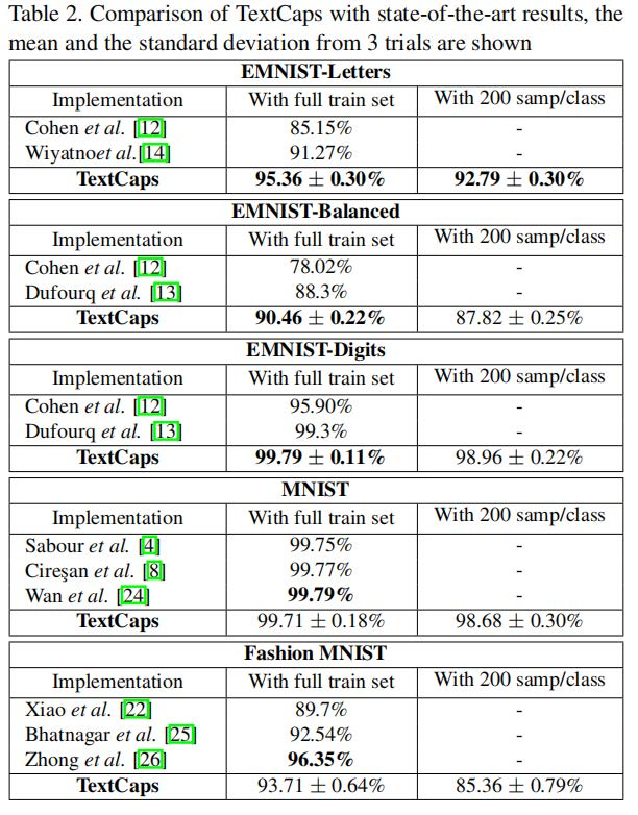
\includegraphics[scale = 1]{Fig/results.pdf}
	\caption{实验结果与对比图}
	\label{fig:results}
\end{figure}






